\chapter{Background and previous work}
% % One of the major problems in data analysis is the interaction of sets of discrete points with each other and how to obtain high-dimensional structures from low-dimensional representations. Classical analysis does not answer the question of how to study not individual points, but entire structures consisting of them. One of methods for solving this problem lies in algebraic topology. A separate section of data science is devoted to this method - topological data analysis. One of the main tasks of TDA is to extract information from data sets that are high-dimensional, incomplete and noisy. Topology allows you to define the relationship between discrete sets of variables and continuous images, thereby expanding the data into a continuous image that will be perceived as a single scene.

% % To understand how it works, we need to introduce several definitions. 
% We will call a point cloud -- a finite set of points in some Euclidean space $\mathbb{R}^{n}$. 
% % One of the most important type of point clouds in our case is be the data set coming from the image of real objects in space. Data about such an object is determined by point from line lasers scan a body in space and explore the surface and specifying the coordinates of points on the surface of selected body.

% To calculate homologies numerically we use simplicial complexes. These are combinatorial objects that define the structure of spatial data using analog $n$-dimensional simplices for different sets.

% \begin{definition}
%     Simplicial complex on the finite set of points $A$  -- 
%  collection of subsets $K \subset 2^A$ of set $A$,when the following conditions are met:
 
%  1) if $I \in K$ and $J \subset I$, than $J \in K$
 
%  2)  $\emptyset \in K$ 

%  Element of $K$ will call simplexes, $A$ -- the set of vertex, and we will say that $i$ the vertex of simplexes $I$, if $i \in I$. Dimension of simplex is number $|I| - 1$.
% \end{definition}

% Easy to see that simlicial complex with simplexes dimentions $\leq 1$ is graph. and if we start pasting high-dimensional simplices onto it, we get a flat image of the simlicial complex. 

% for calculations we will use Rips complex

% \begin{definition}
%    Rips complex for collection of points $\{x_{\alpha}\}$ in Euclidean space -- the abstract simlicial complex whose $k$-simplices are determined by unordered $(k-1)$-tuples of points $\{x_{\alpha}\}^k_0$ which are pairwise  within distance $\varepsilon$.
% \end{definition}

% Thus, we have determined the complex with which we will work. But to study the topological structure, homologies are used, they allow to look at the rougher properties of an object and are more resistant to point movements.

% Stable homology is a multiscale analogue of the homology group, which contains information about changes in topological features when filtering spaces. While the regular homology group represents the non-trivial homology classes of a particular topological space, the constant homology group allows the study of only those classes that remain non-trivial across a variety of basic filtering parameters.

% \begin{definition}
% The persistent homology group ${\displaystyle PH}$ of a point cloud is the persistence module defined as ${\displaystyle PH_{k}(X)=\prod H_{k}(X_{\varepsilon})}$, where ${\displaystyle X_{\varepsilon}}$ is the Rips complex of radius ${\displaystyle \varepsilon}$ of the point cloud ${\displaystyle X}$ and ${\displaystyle H_{k}}$ is the homology group.
% \end{definition}



% Let's sample from two distributions \textgoth{P} and \textgoth{Q} two point clouds $P = \{p_i\}$, and $Q = \{q_j\}$, such that $p_i$, $q_j$ $ \in \mathbb{R}^d$. 
% Than in order to define Cross-Barcode$(P, Q)$ we will firstly construct the following filtered simplicial complex. 
% Let $(\Gamma_{P \cup Q}, m_{P \cup Q/Q})$ be the weighted graph constructed in the following way.
% Set of vertexes is equal to union of points of $P$ and $Q$.
% Set of edges is defined by distance matrix consisting of pairwise distances between all pairs of vertexes of the form $(p_i,p_j)$ or $(p_i, q_j)$ factor Q in this context means that we set all distances in pairs of form $(q_i, q_j)$ are set to be equal zero.
% Our filtered simplicial complex is the Vietoris-Rips complex of $(\Gamma_{P \cup Q}, m_{P \cup Q/Q})$.

% Note that, using a weighted graph, the Vietoris-Rips complex is constructed as follows: given a real parameter, for each of its values, $R_{\alpha}(\Gamma, m)$ consist of simplices formed by subsets of vertices where all pairwise distances between these vertices do not exceed $\alpha$ according to $m$.
% Increasing the value of $\alpha$ adds more simplices and this gives a nested family of collections of simplices know as filtered simplicial complex. 

% In addition let us remind that that a simplicial complex is described by a set of vertices $V = \{v_1, ... , v_N\}$, and a collection of $(k + 1)$-elements its subsets named k-simplices for $k \ge 0$. 
% All that is required is that for any simplex in S (set of simlices) it is true that all its faces are of lower dimension, i.e. any subset of its vertices must also be contained in a set of simplexes of a complex.

% The filtered simplicial complexes is the family of simplicial complexes $S_{\alpha}$ with nested collections of simplices: for $\alpha_1$ < $\alpha_2$ all simplices of $S_{\alpha_1}$ are also in $S_{\alpha_2}$.
% When parameter $\alpha$ is equal to zero, the simplicial complex $R_{\alpha}(\Gamma_{P \cup Q}, m_{P \cup Q)/Q})$ has trivial homology $H_k$ for all k > 0 since it contains all simplices formed by Q-points and no other simplices. 

% The dimension of the 0-th homology equals at $\alpha$ = 0 to the number of P-points plus one, since no edge between them or between a P-point and a Q-point is added at the beginning. 
% As we increase the value of parameter $\alpha$, there vill appers a bunch of cycles and holes in the Vietoris-Rips complex. 
% Then, during the growth of $\alpha$ some combinations of these cycles will disappear. 

% The persistent homology principal theorem (!!!) implies that it is possible to choose the set of generators in the homology of filtered complexes $H_k(R_{\alpha})$ across all the scales $\alpha$ such that each generator appears at its specific "birth" time and disappears at its specific "death" time. These sets of “birth" and “deaths" of topological features in $R_{\alpha}$ are registered in Barcode of the filtered complex.

% \begin{definition} 
% The Cross-Barcode$(P, Q)_i$ is the set of intervals recording the “births" and “deaths" times of $i$-dimensional topological features in the filtered simplicial complex 
% \end{definition}

% $R_{\alpha}(\Gamma_{P \cup Q}, m_{P \cup Q)/Q})$.

% Examples of Cross-Barcodes are shown on Fig (!!!). 
% Topological holes which stay alive for the longest timeperiod are considered essential. The topological features with “birth" time equal to “death" time are trivial by definition and do not appear in Cross-Barcode.

% There are three important properties of barcodes.

% \begin{itemize}
%   \item If P is equal to Q as clouds Cross-Barcode$(P, Q)$ = Cross-Barcode$(P, P)$ = $\varnothing$.
%   \item If $Q = \varnothing$ Cross-Barcode$(P, Q)$ = Barcode$(P)$ - barcode of single point cloud P.
%   \item The norm of i-th component of barcode (in terms of time before trivialization) can be bounded by Hausdorff distance between P and Q. 
% \end{itemize}

% \paragraph{The Manifold Topology Divergence}

% The bound from previos statement and the equality Cross-Barcode$(P, P)$ to $\varnothing$ imply that the closeness of Cross-Barcode(P, Q) to the empty set is a natural measure of discrepancy between P and Q. 


% Each Cross-Barcode$(P, Q)_i$ is a list of intervals describing the persistent homology $H_i$.

% Thus, to understand how close we are to the empty set we can use a large number of different characteristics such ass: sum or sum of squared lengths, number of segments, the maximal length ($H_i$ max) or specific quantile. 

% Various characteristics of high-dimensional homology can be used for different tasks; however, it should be noted that the cross-barcodes for $H_0$ and $H_1$ can be calculated relatively fast.

% So MTop-Divergence$(P, Q)$ is based on the sum of lengths of segments in 

% Cross-Barcode$(P, Q)_1$, see (!!!) for details. 
% In addition, there is a different interpretation of the sum of lengths of segments in Cross-Barcode$(P, Q)_1$ related to the Earth Mover’s Distance. 

% Namely, it can be proved that (!!!) that Earth Mover’s Distance between the Relative Living Time histogram for Cross-Barcode$(P, Q)_1$ and the histogram of the empty barcode, multiplied by the parameter $\alpha_{max}$ see (!!!), is equal to the sum of lengths of segments in $H_1$. 
% This explains the good stability properties of this quantity.

% This metrics can be applied mainly in two settings: to a pair of distributions $\textgoth{P}_data$, $\textgoth{Q}_model$, in which case can be denoted score MTop-Div$(\textgoth{P}, \textgoth{Q})$, and to a pair of distributions $\textgoth{Q}_model$, $\textgoth{P}_data$, in which case score is denoted MTop-Div$(\textgoth{M}, \textgoth{D})$. 

% These two variants of the Cross-Barcode, and of the MTopDivergence are related to the concepts of precision and recall. 

% These two variants can be analyzed
% separately or combined together, e.g. averaged.

\section{Proposed loss} There are a handful of ways to compute continuous topological quantities that help distinguish structures within point clouds or compare point clouds to measure similarity or even you as an objective function for optimization purposes. We will discuss some of them below, but let's first discuss the loss quantity we will use throughout our experiments. Following the notation from \cite{MTopDiv}, for a given graph $G$ we will denote an ordered collection of lengths of edges om Minimal Spanning Tree of $G$ as Barcode${}_0$. Sum of those values (total weight of minimal spanning tree) will be our loss. It's that simple. The interesting properties arise from the way one constructs graph $G$ and measures distances between points. If we just optimize such a sum, we minimize number of connected components and overall size of structure a little bit too \ref{fig:optimizel1} which gives us the idea of method \ref{algo:reg}

\begin{figure}[h!]
    \centering
    \begin{subfigure}{.5\textwidth}
  \centering
  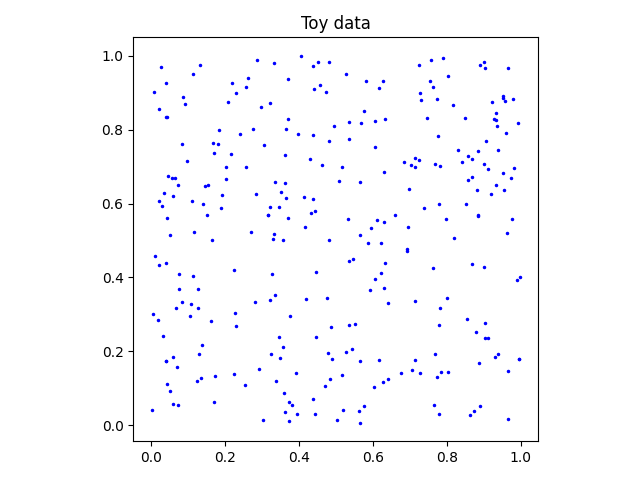
\includegraphics[width=\textwidth]{images/opt/toydata.png}
  \caption{At initialization}
  \label{fig:sub1}
\end{subfigure}%
\begin{subfigure}{.5\textwidth}
  \centering
  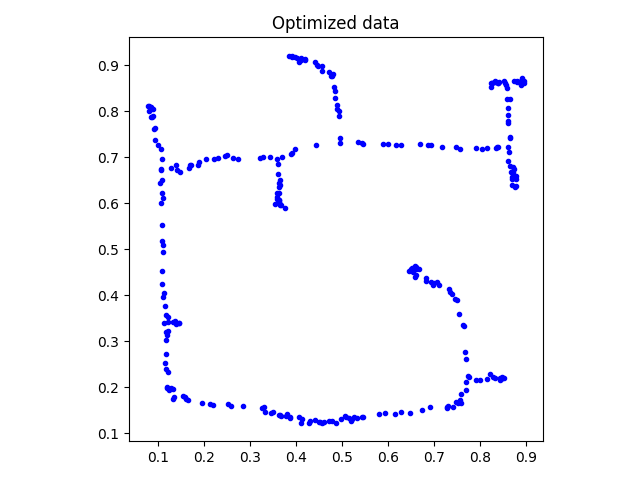
\includegraphics[width=\textwidth]{images/opt/optdata.png}
  \caption{Optimization result}
  \label{fig:sub2}
\end{subfigure}
    \caption{Optimizing $\ell_1$ for a set of 2d points improved simple connectivity of point cloud}
    \label{fig:optimizel1}
\end{figure}

If for a graph we unite two point clouds, but contract all the edges within one of them we obtain Cross-Barcode cleverly defined in \cite{MTopDiv}. Sum of lengths in Cross-Barcode${}_0$ allows us to measure (asymmetric) discrepancy between two point clouds, which we call MTop-Div${}_{0}$ similarly to the seminal paper and use it to regularize GANs. Efficient and scalable implementation for finding MST (aka Kruskal algorithm) is available \cite{Hofer17a, Hofer19a} and our experiments rely on it heavily.

\section{Similar approaches}
\begin{itemize}
    \item in TopoAE \cite{moor2021topological} authors compute barcodes for input batch treated as point cloud, then for latent representation and use MSE between barcodes to formulate a regularization term
    \item in \cite{Hofer19a} authors compute barcodes for latent representation of a given point cloud (after applying encoder) and enforce connectivity by  imposing MAE between barcode and given small number (so all essential edges converge towards given length)
    \item in \cite{topo-segm} and several similar works, first-order barcodes are computed from persistent homologies of 2-dimensional scalar signal (segmentation map of given image) and loss is Earth Mover's distance between between target and predicted mask barcodes
    \item \cite{balabin2024disentanglement} also train (variational) autoencoder, but regularize difference between latent descriptors of original and augmented data using Representation Topology Divergence \cite{rtd}, a closely related methodology of topologically comparing point clouds with one-to-one correspondence
\end{itemize}
To the best of authors knowledge no work has been done to apply topological regularizers for Gaussian Splatting and point cloud based 3d scene reconstructions.
